\section{Arrikto's Rok}

Rok provides an enterprise data management layer that allows users to instantly
snapshot their containers for local and offsite backup, take immutable,
consistent snapshots of their apps and keep them in a backup store, e.g., Amazon
S3. It allows users to snapshot, version, package, distribute, and clone their
entire environment along with its data. It is natively integrated with
Kubernetes as one of its supported platforms.

\begin{figure}[ht]
    \centering
    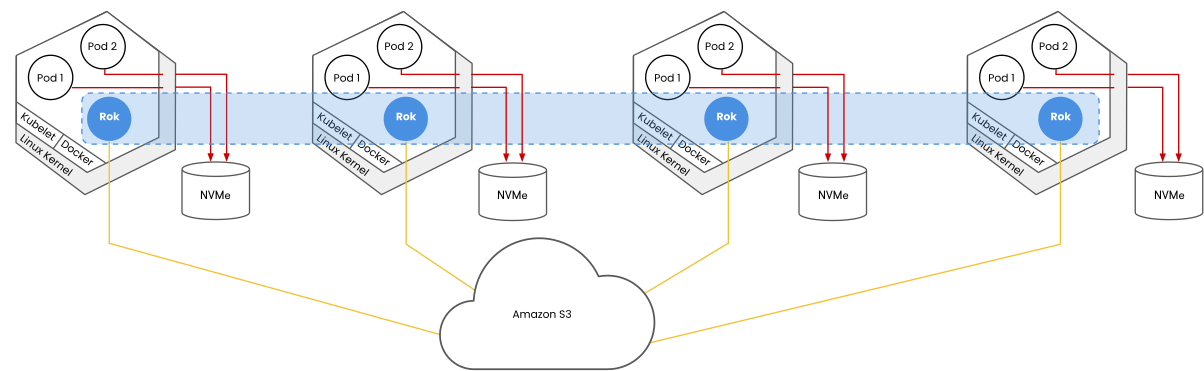
\includegraphics[width=\textwidth]{resources/rok-cluster-f.pdf}
    \caption{A Rok Cluster}
\end{figure}

\subsection{The Rok Operator}
\label{section:background-rok-operator}

Rok clusters ship with the \textit{Rok operator}, a component that implements
the Kubernetes \textit{operator} pattern (see section
\ref{section:operator-pattern}) and manages the Rok cluster. Rok Operator
watches the \co{rokCluster} Custom Resource and takes any actions required to
bring the state of the cluster to the desired state. 

The Rok operator is responsible
--among others-- for deploying the Rok CSI driver on the cluster and managing
the Rok CSI data protection mechanism (Rok CSI Guards), which we will explain in
the next chapter.

\subsection{The Rok Storage System}
\label{section:background-rok-csi}

The Rok storage system gathers the available local NVMe disks attached to a node
and, using LVM, aggregates them into a single Volume Group, hereafter referred
to as the ``\textit{Rok VG}''. The Rok VG is the storage place where Rok
dynamically provisions the requested volumes.

Rok's storage driver integrates with Kubernetes by implementing the Container
Storage Interface. We will refer to the Rok's storage driver as the
``\textit{Rok CSI}''. The Rok CSI follows the CSI plugins architecture and is
deployed on the cluster as the following Kubernetes resources:
\begin{itemize}
    \item A DaemonSet, running on every node the CSI Node plugin, hereafter
    referred to as the ``\textit{Rok CSI Node}''. The Rok CSI Node handles the
    provisioning and the management of the local volumes on each node. The Pod
    of the Rok CSI Node consists of the CSI Node service container and the Node
    Driver Registrar sidecar.
    \item A StatefulSet, running the Controller plugin on an arbitrary node,
    hereafter referred to as the ``Rok CSI Controller''. The Pod of the Rok CSI
    Controller consists of the CSI Controller service container, the external
    attacher, and the external provisioner sidecars.
\end{itemize}

The architecture of the Rok CSI storage system is illustrated in Figure
\ref{figure:rok-csi-architecture}.

\begin{figure}[ht]
  \centering
  \includegraphics[width=0.9\textwidth]{resources/rok-csi-architecture.pdf}
  \caption{The architecture of the Rok storage system}
  \label{figure:rok-csi-architecture}
\end{figure}